% Supplementary experimental results for Chapter 5
% Expected packages in the main document: graphicx, float, subcaption, booktabs, amsmath, placeins
% The main document should enter appendix mode with \appendix before inputting this file.

\chapter{Supplementary Experimental Material}
\label{app:supplementary-results}

This appendix collects supplementary experimental material used to support the
comparisons in Chapter~\ref{chap:results}. It is intentionally selective: the
main text keeps only the figures needed for the central empirical narrative,
while the material below provides alternative normalizations, broader learner
coverage, pairwise comparisons, horizon-scaling fits, and selected repeated-game
profiles where these make the reported comparisons easier to verify. Unless stated otherwise, the
experimental configuration is the same as in Chapter~\ref{chap:results}.

\clearpage
% ============================================================
\section{One-Player Results}
\label{app:one-player-results}

\subsection{Root-T Normalized Trajectories}
\label{app:one-player-trajectories}

The \(R_T/\sqrt{T}\) normalization is shown here for the aggregate
swap-regret comparison and for the RM / SRM pairwise comparison.

\begin{figure}[htbp]
    \centering
    \begin{subfigure}{0.47\textwidth}
        \centering
        \includegraphics[page=12,width=\linewidth]{figures/regret/hfa/algorithm_comparison_full_information.pdf}
        \caption{HFA, full information}
    \end{subfigure}\hfill
    \begin{subfigure}{0.47\textwidth}
        \centering
        \includegraphics[page=12,width=\linewidth]{figures/regret/hfa/algorithm_comparison_bandit.pdf}
        \caption{HFA, bandit}
    \end{subfigure}

    \begin{subfigure}{0.47\textwidth}
        \centering
        \includegraphics[page=12,width=\linewidth]{figures/regret/lrw/algorithm_comparison_full_information.pdf}
        \caption{LRW, full information}
    \end{subfigure}\hfill
    \begin{subfigure}{0.47\textwidth}
        \centering
        \includegraphics[page=12,width=\linewidth]{figures/regret/lrw/algorithm_comparison_bandit.pdf}
        \caption{LRW, bandit}
    \end{subfigure}
    \caption{Swap regret under \(R_T/\sqrt{T}\) in both one-player environments.}
    \label{fig:app-oneplayer-swap-sqrt}
\end{figure}

\begin{figure}[htbp]
    \centering

    \begin{subfigure}{0.43\textwidth}
        \centering
        \includegraphics[page=4,width=\linewidth]
        {figures/regret/hfa/regret_matching_comparison.pdf}
        \caption{HFA, external regret}
    \end{subfigure}\hfill
    \begin{subfigure}{0.43\textwidth}
        \centering
        \includegraphics[page=4,width=\linewidth]
        {figures/regret/lrw/regret_matching_comparison.pdf}
        \caption{LRW, external regret}
    \end{subfigure}

    \begin{subfigure}{0.43\textwidth}
        \centering
        \includegraphics[page=8,width=\linewidth]
        {figures/regret/hfa/regret_matching_comparison.pdf}
        \caption{HFA, internal regret}
    \end{subfigure}\hfill
    \begin{subfigure}{0.43\textwidth}
        \centering
        \includegraphics[page=8,width=\linewidth]
        {figures/regret/lrw/regret_matching_comparison.pdf}
        \caption{LRW, internal regret}
    \end{subfigure}

    \begin{subfigure}{0.43\textwidth}
        \centering
        \includegraphics[page=12,width=\linewidth]
        {figures/regret/hfa/regret_matching_comparison.pdf}
        \caption{HFA, swap regret}
    \end{subfigure}\hfill
    \begin{subfigure}{0.43\textwidth}
        \centering
        \includegraphics[page=12,width=\linewidth]
        {figures/regret/lrw/regret_matching_comparison.pdf}
        \caption{LRW, swap regret}
    \end{subfigure}

    \caption{RM and SRM under \(R_T/\sqrt{T}\) in both one-player environments.}
    \label{fig:app-rm-srm-sqrt}
\end{figure}

\FloatBarrier

% ------------------------------------------------------------
\clearpage
\subsection{Individual Horizon-Scaling Fits}
\label{app:horizon-scaling}

The following panels show the individual independent-horizon fits summarized
by Table~\ref{tab:regret-scaling}. Algorithms follow the same order as in the
table, with HFA shown in the left column and LRW in the right column. The page
breaks are used only for layout.

\begin{figure}[H]
    \centering

    \begin{subfigure}{0.47\textwidth}\centering
        \includegraphics[page=6,width=\linewidth,height=0.18\textheight,keepaspectratio]{figures/regret/hfa/horizon_scaling_full_information.pdf}
        \caption{HFA, Hedge}
    \end{subfigure}\hfill
    \begin{subfigure}{0.47\textwidth}\centering
        \includegraphics[page=6,width=\linewidth,height=0.18\textheight,keepaspectratio]{figures/regret/lrw/horizon_scaling_full_information.pdf}
        \caption{LRW, Hedge}
    \end{subfigure}

    \begin{subfigure}{0.47\textwidth}\centering
        \includegraphics[page=10,width=\linewidth,height=0.18\textheight,keepaspectratio]{figures/regret/hfa/horizon_scaling_full_information.pdf}
        \caption{HFA, OptHedge}
    \end{subfigure}\hfill
    \begin{subfigure}{0.47\textwidth}\centering
        \includegraphics[page=10,width=\linewidth,height=0.18\textheight,keepaspectratio]{figures/regret/lrw/horizon_scaling_full_information.pdf}
        \caption{LRW, OptHedge}
    \end{subfigure}

    \begin{subfigure}{0.47\textwidth}\centering
        \includegraphics[page=2,width=\linewidth,height=0.18\textheight,keepaspectratio]{figures/regret/hfa/horizon_scaling_full_information.pdf}
        \caption{HFA, BM-Hedge}
    \end{subfigure}\hfill
    \begin{subfigure}{0.47\textwidth}\centering
        \includegraphics[page=2,width=\linewidth,height=0.18\textheight,keepaspectratio]{figures/regret/lrw/horizon_scaling_full_information.pdf}
        \caption{LRW, BM-Hedge}
    \end{subfigure}

    \caption{Independent-horizon fits for the algorithms in Table~\ref{tab:regret-scaling}.}
    \label{fig:app-horizon-scaling-details}
\end{figure}

\clearpage

\begin{figure}[H]
    \ContinuedFloat
    \captionsetup{list=no}
    \centering

    \begin{subfigure}{0.47\textwidth}\centering
        \includegraphics[page=4,width=\linewidth,height=0.17\textheight,keepaspectratio]{figures/regret/hfa/horizon_scaling_full_information.pdf}
        \caption{HFA, BM-OptHedge}
    \end{subfigure}\hfill
    \begin{subfigure}{0.47\textwidth}\centering
        \includegraphics[page=4,width=\linewidth,height=0.17\textheight,keepaspectratio]{figures/regret/lrw/horizon_scaling_full_information.pdf}
        \caption{LRW, BM-OptHedge}
    \end{subfigure}

    \begin{subfigure}{0.47\textwidth}\centering
        \includegraphics[page=8,width=\linewidth,height=0.17\textheight,keepaspectratio]{figures/regret/hfa/horizon_scaling_full_information.pdf}
        \caption{HFA, Ito-Hedge}
    \end{subfigure}\hfill
    \begin{subfigure}{0.47\textwidth}\centering
        \includegraphics[page=8,width=\linewidth,height=0.17\textheight,keepaspectratio]{figures/regret/lrw/horizon_scaling_full_information.pdf}
        \caption{LRW, Ito-Hedge}
    \end{subfigure}

    \begin{subfigure}{0.47\textwidth}\centering
        \includegraphics[page=12,width=\linewidth,height=0.17\textheight,keepaspectratio]{figures/regret/hfa/horizon_scaling_full_information.pdf}
        \caption{HFA, RM}
    \end{subfigure}\hfill
    \begin{subfigure}{0.47\textwidth}\centering
        \includegraphics[page=12,width=\linewidth,height=0.17\textheight,keepaspectratio]{figures/regret/lrw/horizon_scaling_full_information.pdf}
        \caption{LRW, RM}
    \end{subfigure}

    \begin{subfigure}{0.47\textwidth}\centering
        \includegraphics[page=14,width=\linewidth,height=0.17\textheight,keepaspectratio]{figures/regret/hfa/horizon_scaling_full_information.pdf}
        \caption{HFA, SRM}
    \end{subfigure}\hfill
    \begin{subfigure}{0.47\textwidth}\centering
        \includegraphics[page=14,width=\linewidth,height=0.17\textheight,keepaspectratio]{figures/regret/lrw/horizon_scaling_full_information.pdf}
        \caption{LRW, SRM}
    \end{subfigure}

    \caption{Independent-horizon fits (continued).}
\end{figure}

\clearpage

\begin{figure}[H]
    \ContinuedFloat
    \captionsetup{list=no}
    \centering

    \begin{subfigure}{0.47\textwidth}\centering
        \includegraphics[page=2,width=\linewidth,height=0.145\textheight,keepaspectratio]{figures/regret/hfa/horizon_scaling_bandit.pdf}
        \caption{HFA, EXP3}
    \end{subfigure}\hfill
    \begin{subfigure}{0.47\textwidth}\centering
        \includegraphics[page=2,width=\linewidth,height=0.145\textheight,keepaspectratio]{figures/regret/lrw/horizon_scaling_bandit.pdf}
        \caption{LRW, EXP3}
    \end{subfigure}

    \begin{subfigure}{0.47\textwidth}\centering
        \includegraphics[page=6,width=\linewidth,height=0.145\textheight,keepaspectratio]{figures/regret/hfa/horizon_scaling_bandit.pdf}
        \caption{HFA, EXP3-IX}
    \end{subfigure}\hfill
    \begin{subfigure}{0.47\textwidth}\centering
        \includegraphics[page=6,width=\linewidth,height=0.145\textheight,keepaspectratio]{figures/regret/lrw/horizon_scaling_bandit.pdf}
        \caption{LRW, EXP3-IX}
    \end{subfigure}

    \begin{subfigure}{0.47\textwidth}\centering
        \includegraphics[page=4,width=\linewidth,height=0.145\textheight,keepaspectratio]{figures/regret/hfa/horizon_scaling_bandit.pdf}
        \caption{HFA, BM-EXP3}
    \end{subfigure}\hfill
    \begin{subfigure}{0.47\textwidth}\centering
        \includegraphics[page=4,width=\linewidth,height=0.145\textheight,keepaspectratio]{figures/regret/lrw/horizon_scaling_bandit.pdf}
        \caption{LRW, BM-EXP3}
    \end{subfigure}

    \begin{subfigure}{0.47\textwidth}\centering
        \includegraphics[page=8,width=\linewidth,height=0.145\textheight,keepaspectratio]{figures/regret/hfa/horizon_scaling_bandit.pdf}
        \caption{HFA, Ito-Tsallis}
    \end{subfigure}\hfill
    \begin{subfigure}{0.47\textwidth}\centering
        \includegraphics[page=8,width=\linewidth,height=0.145\textheight,keepaspectratio]{figures/regret/lrw/horizon_scaling_bandit.pdf}
        \caption{LRW, Ito-Tsallis}
    \end{subfigure}

    \begin{subfigure}{0.47\textwidth}\centering
        \includegraphics[page=10,width=\linewidth,height=0.145\textheight,keepaspectratio]{figures/regret/hfa/horizon_scaling_bandit.pdf}
        \caption{HFA, LCE-IX}
    \end{subfigure}\hfill
    \begin{subfigure}{0.47\textwidth}\centering
        \includegraphics[page=10,width=\linewidth,height=0.145\textheight,keepaspectratio]{figures/regret/lrw/horizon_scaling_bandit.pdf}
        \caption{LRW, LCE-IX}
    \end{subfigure}

    \caption{Independent-horizon fits (continued).}
\end{figure}

\FloatBarrier

% ------------------------------------------------------------
\clearpage
\subsection{Action-Space Scaling Examples}
\label{app:action-space-scaling}

Figure~\ref{fig:app-action-space-selected} provides selected additional
examples for the action-space effect discussed in
Section~\ref{sec:action-space-scaling-results}.

\begin{figure}[H]
    \centering

    \begin{subfigure}{0.43\textwidth}
        \centering
        \includegraphics[
            page=2,
            width=\linewidth
        ]{figures/regret/hfa/action_space_scaling_full_information.pdf}
        \caption{BM-Hedge, external regret}
    \end{subfigure}
    \hfill
    \begin{subfigure}{0.43\textwidth}
        \centering
        \includegraphics[
            page=10,
            width=\linewidth
        ]{figures/regret/hfa/action_space_scaling_full_information.pdf}
        \caption{BM-Hedge, swap regret}
    \end{subfigure}

    \begin{subfigure}{0.43\textwidth}
        \centering
        \includegraphics[
            page=14,
            width=\linewidth
        ]{figures/regret/hfa/action_space_scaling_bandit.pdf}
        \caption{BM-EXP3, external regret}
    \end{subfigure}
    \hfill
    \begin{subfigure}{0.43\textwidth}
        \centering
        \includegraphics[
            page=22,
            width=\linewidth
        ]{figures/regret/hfa/action_space_scaling_bandit.pdf}
        \caption{BM-EXP3, swap regret}
    \end{subfigure}

    \begin{subfigure}{0.43\textwidth}
        \centering
        \includegraphics[
            page=38,
            width=\linewidth
        ]{figures/regret/hfa/action_space_scaling_bandit.pdf}
        \caption{Ito-Tsallis, external regret}
    \end{subfigure}
    \hfill
    \begin{subfigure}{0.43\textwidth}
        \centering
        \includegraphics[
            page=46,
            width=\linewidth
        ]{figures/regret/hfa/action_space_scaling_bandit.pdf}
        \caption{Ito-Tsallis, swap regret}
    \end{subfigure}

    \caption{Action-space scaling for BM-Hedge, BM-EXP3, and Ito-Tsallis in the historical-frequency environment.}
    \label{fig:app-action-space-selected}
\end{figure}

\FloatBarrier

% ============================================================
\clearpage
\section{Repeated-Game Results}
\label{app:repeated-game-results}

\subsection{RPSLS Self-Play Regret Trajectories}
\label{app:rpsls-selfplay-regret}

The panels supplement Table~\ref{tab:rpsls-selfplay-summary} with player~0
external-, internal-, and swap-regret trajectories for RPSLS self-play under
both feedback models.

\begin{figure}[H]
    \centering

    \begin{subfigure}{0.38\textwidth}\centering
        \includegraphics[page=2,width=\linewidth]{figures/games/rpsls/selfplay_regret_full_information.pdf}
        \caption{External regret, $R_T/T$}
    \end{subfigure}\hfill
    \begin{subfigure}{0.38\textwidth}\centering
        \includegraphics[page=4,width=\linewidth]{figures/games/rpsls/selfplay_regret_full_information.pdf}
        \caption{External regret, $R_T/\sqrt{T}$}
    \end{subfigure}

    \begin{subfigure}{0.38\textwidth}\centering
        \includegraphics[page=6,width=\linewidth]{figures/games/rpsls/selfplay_regret_full_information.pdf}
        \caption{Internal regret, $R_T/T$}
    \end{subfigure}\hfill
    \begin{subfigure}{0.38\textwidth}\centering
        \includegraphics[page=8,width=\linewidth]{figures/games/rpsls/selfplay_regret_full_information.pdf}
        \caption{Internal regret, $R_T/\sqrt{T}$}
    \end{subfigure}

    \begin{subfigure}{0.38\textwidth}\centering
        \includegraphics[page=10,width=\linewidth]{figures/games/rpsls/selfplay_regret_full_information.pdf}
        \caption{Swap regret, $R_T/T$}
    \end{subfigure}\hfill
    \begin{subfigure}{0.38\textwidth}\centering
        \includegraphics[page=12,width=\linewidth]{figures/games/rpsls/selfplay_regret_full_information.pdf}
        \caption{Swap regret, $R_T/\sqrt{T}$}
    \end{subfigure}

    \caption{RPSLS self-play regret for player~0 under full-information feedback at $T=10^6$.}
    \label{fig:app-rpsls-selfplay-regret-full}
\end{figure}

\begin{figure}[H]
    \centering

    \begin{subfigure}{0.38\textwidth}\centering
        \includegraphics[page=2,width=\linewidth]{figures/games/rpsls/selfplay_regret_bandit.pdf}
        \caption{External regret, $R_T/T$}
    \end{subfigure}\hfill
    \begin{subfigure}{0.38\textwidth}\centering
        \includegraphics[page=4,width=\linewidth]{figures/games/rpsls/selfplay_regret_bandit.pdf}
        \caption{External regret, $R_T/\sqrt{T}$}
    \end{subfigure}

    \begin{subfigure}{0.38\textwidth}\centering
        \includegraphics[page=6,width=\linewidth]{figures/games/rpsls/selfplay_regret_bandit.pdf}
        \caption{Internal regret, $R_T/T$}
    \end{subfigure}\hfill
    \begin{subfigure}{0.38\textwidth}\centering
        \includegraphics[page=8,width=\linewidth]{figures/games/rpsls/selfplay_regret_bandit.pdf}
        \caption{Internal regret, $R_T/\sqrt{T}$}
    \end{subfigure}

    \begin{subfigure}{0.38\textwidth}\centering
        \includegraphics[page=10,width=\linewidth]{figures/games/rpsls/selfplay_regret_bandit.pdf}
        \caption{Swap regret, $R_T/T$}
    \end{subfigure}\hfill
    \begin{subfigure}{0.38\textwidth}\centering
        \includegraphics[page=12,width=\linewidth]{figures/games/rpsls/selfplay_regret_bandit.pdf}
        \caption{Swap regret, $R_T/\sqrt{T}$}
    \end{subfigure}

    \caption{RPSLS self-play regret for player~0 under bandit feedback at $T=10^6$.}
    \label{fig:app-rpsls-selfplay-regret-bandit}
\end{figure}

\FloatBarrier

% ------------------------------------------------------------
\clearpage
\subsection{Selected RPS and RPSLS Equilibrium Profiles}
\label{app:rps-equilibrium-profiles}

The panels below complement Section~\ref{sec:joint-action-structure} with
joint-action distributions and CE/CCE distance trajectories for EXP3 and
EXP3-IX in RPS, and for Hedge in RPSLS.

\begin{figure}[H]
    \centering

    \begin{subfigure}{0.43\textwidth}\centering
        \includegraphics[page=2,width=\linewidth]{figures/games/rps/equilibrium_bandit.pdf}
        \caption{RPS, EXP3, joint actions}
    \end{subfigure}\hfill
    \begin{subfigure}{0.43\textwidth}\centering
        \includegraphics[page=4,width=\linewidth]{figures/games/rps/equilibrium_bandit.pdf}
        \caption{RPS, EXP3, CE/CCE distance}
    \end{subfigure}

    \begin{subfigure}{0.43\textwidth}\centering
        \includegraphics[page=10,width=\linewidth]{figures/games/rps/equilibrium_bandit.pdf}
        \caption{RPS, EXP3-IX, joint actions}
    \end{subfigure}\hfill
    \begin{subfigure}{0.43\textwidth}\centering
        \includegraphics[page=12,width=\linewidth]{figures/games/rps/equilibrium_bandit.pdf}
        \caption{RPS, EXP3-IX, CE/CCE distance}
    \end{subfigure}

    \begin{subfigure}{0.43\textwidth}\centering
        \includegraphics[page=10,width=\linewidth]{figures/games/rpsls/equilibrium_selfplay_full_information.pdf}
        \caption{RPSLS, Hedge, joint actions}
    \end{subfigure}\hfill
    \begin{subfigure}{0.43\textwidth}\centering
        \includegraphics[page=12,width=\linewidth]{figures/games/rpsls/equilibrium_selfplay_full_information.pdf}
        \caption{RPSLS, Hedge, CE/CCE distance}
    \end{subfigure}

    \caption{Joint-action distributions and CE/CCE distances for EXP3 and EXP3-IX in RPS and Hedge in RPSLS self-play.}
    \label{fig:app-rps-external-equilibrium-selected}
\end{figure}

\FloatBarrier

% ------------------------------------------------------------
\clearpage
